\section{Estructura Organizacional} \label{sect:Estructura_organizacional}

Empresas TD es una compañía con una gran proyección a futuro compuesta mayormente 
por gente joven. El perfil buscado en los miembros del equipo de trabajo es el de 
un profesional dinámico, creativo e innovador, comprometido por brindar a los
asociados y usuarios experiencias de alta calidad. 

Actualmente se gestionan cuatro proyectos en Empresas TD, como se puede ver en la figura \ref{fig:ogtd} y se describen a continuación:

\begin{figure}[h]
	\begin{center}
		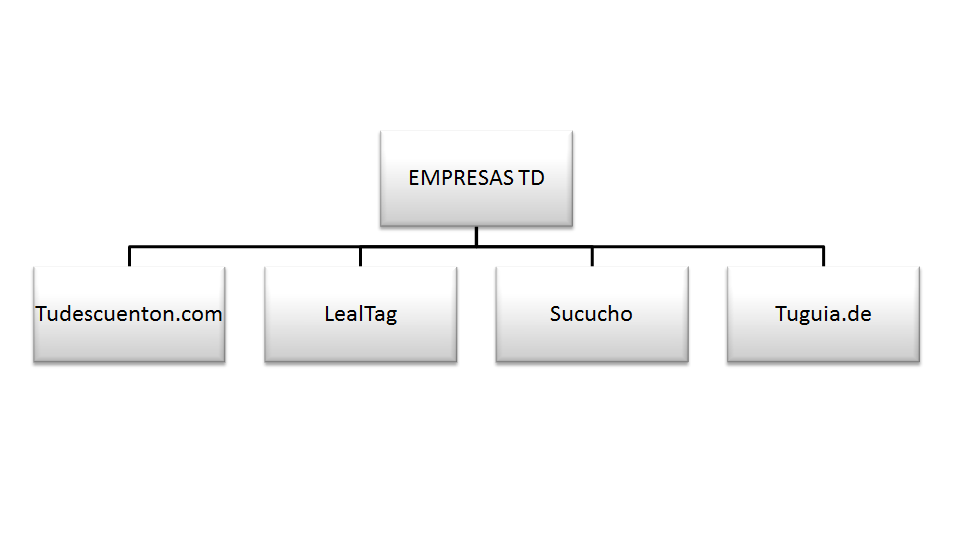
\includegraphics[scale=0.4]{imagenes/OrganigramaTD.png}
	\end{center}
	\caption{
		\label{fig:ogtd}
		Organigrama de Empresas TD.
	}
\end{figure}

\begin{itemize}
  \item \textbf{Tudescuenton:} es ``una que plataforma le brinda a los venezolanos, la oportunidad de conocer las mejores cosas que hacer, en las principales ciudades del país, a través de descuentos insuperables.'' \cite{TDC}
  \item \textbf{Lealtag:} ``es la plataforma que te permite recibir premios, descuentos y regalos en tus sitios favoritos por ser un cliente frecuente.''\cite{LTG}
  \item \textbf{Sucucho:} ``ofrece a los creativos venezolanos un espacio en donde pueden exponer su talento ante el país, en el cual brindamos la oportunidad de que cada uno tenga su tiendita propia 365 días al año.''\cite{SCC}.
  \item \textbf{Tuguiade:} `` Tuguía.de es una página que sirve para conectar los locales con sus clientes. Ofreciéndoles a los usuarios información verificada de los mismos y la posibilidad de escribir sobre sus experiencias, subir fotos e intercambiar historias con los otros clientes.''\cite{TGD}. 
\end{itemize}
  
Cada proyecto tiene asignado un director general y un esquema organizacional específico que se ajusta a sus necesidades. En el caso de Tuguia.de, proyecto en el que desarrolló la pasantía durante periodo Abril-Septiembre de 2013, el organigrama se muestra en la figura \ref{fig:ogtgd}. Como se puede observar el pasante fue parte de la coordinación de programación, esta unidad opera bajo la supervisión del Ing. Gianpaolo Valero Gerente del Departamento de Tecnología de Empresas TD y esta a cargo del Lic. Alexander Mayora Líder de Desarrollo del proyecto Tuguia.de.

\begin{figure}[h]
	\begin{center}
		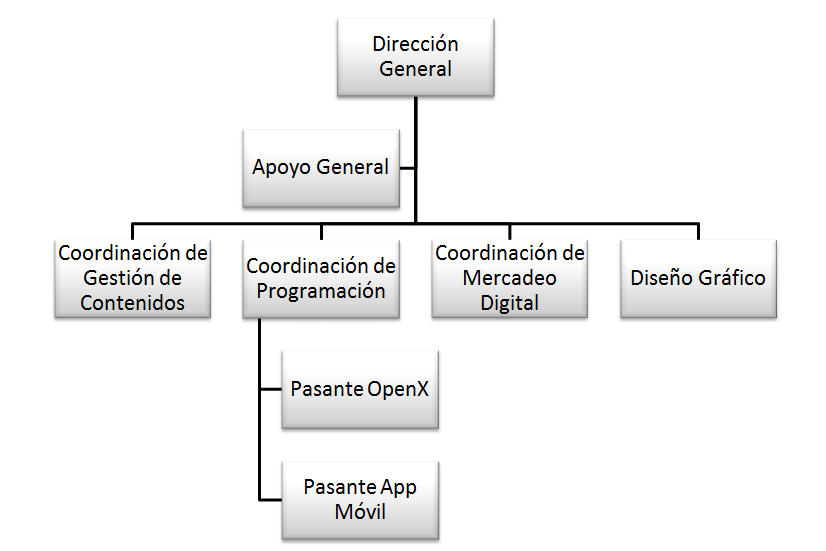
\includegraphics[scale=0.4]{imagenes/OrganigramaTGD.png}
	\end{center}
	\caption{
		\label{fig:ogtgd}
		Organigrama de Tuguia.de
	}
\end{figure}
 